\chapter{Theoretical background}
\section{Artificial neural networks}
An artificial neural network is a computing system inspired by the neural structure of the biological brain and its way of processing information. Such structure is able to ''learn'' how to solve certain problems or recognize patterns without being pre-programmed with rules how to do it. Artificial neural networks are main tool used in  deep learning, which is part of bigger family of machine learning.

\begin{figure}[H]
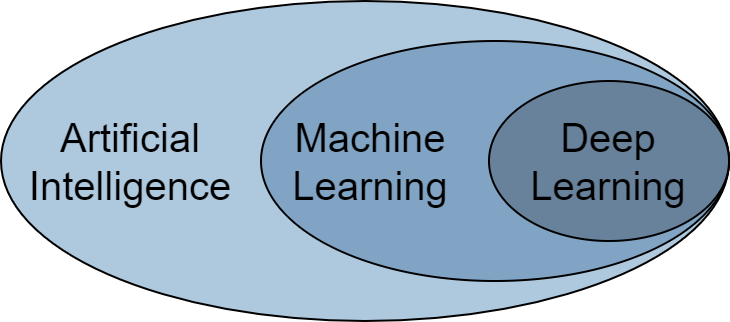
\includegraphics[width=8cm] {deep_learning_chart.png}
\centering
\caption{Deep learning belongingness}
\label{fig:deep_learning_chart}
\end{figure}

\section{Convolutional neural networks}
Explain how it works, what are main use-cases and so on.

\section{Supervised vs unsupervised training}
Description of both and what are main differences and when to use which.